\documentclass[10pt]{article}
\usepackage{commands}


\begin{document}
% Webpage: www.phas.ubc.ca/~seme/526
% Password for webpage: (space)nodrog
\begin{tcolorbox}
  \begin{center}
  \begin{Large}
    \textbf{PHYS 526 (Quantum Field Theory I) Notes} \\
    \vspace{5pt}
  \end{Large}
  \begin{large}
        Rio Weil \\
\vspace{5pt}
    \emph{This document was typeset on \today}
  \end{large}
  \end{center}
\end{tcolorbox}

\begin{center}
  \textbf{Introduction:}

  This is a set of lecture notes taken from UBC's PHYS 526 (Graduate Quantum Field Theory I) course, taught by Dr. Gordon Semenoff. The course covers many-particle systems, second quantization, degenerate Fermi and Bose gases, The action principle and Noether's theorem, Non-relativistic space-time symmetries, relativistic field theories, real scalar quantum field theory, Emergent relativistic symemtry, Dirac field theory, photons, functional methods, and perturbative quantum electrodynamics.  If any errors are found in the notes, feel free to email me at \href{mailto:ryoheiweil@phas.ubc.ca}{ryoheiweil@phas.ubc.ca}.

\end{center}
\addtocontents{toc}{\protect\hypertarget{toc}{}}
\tableofcontents

\newpage
\section{Motivation and Many Particles}

\subsection{Why QFT?}
\begin{enumerate}
    \item Natural way to study QM systems with large number of DOFs
    \item To reconcile special relativity and quantum mechanics (``QM + SR = QFT''). No way to do ``regular'' QM in a relativistic setting. Mainly because $E = mc^2$, so energy can convert into mass; e.g. highly energetic collisions in the LHC which produce a large number of particles. You need a framework which can account for a large type and an arbitrary number of quantum-mechanical particles.
    \item If you take point quantum mechanics and replace the NRQM Hamiltonian (with non-relativistic momentum) with the relativistic version of $H = \sqrt{p^2c^2 + m^2c^4} = mc^2 + \frac{p^2}{2m} + \cdots$, you find that the particle disperses (much like in the non-relativistic case) but it spreads in such a way that it violates causality; i.e. it can disperse outside of the light cone. There is no way to repair this in single-particle point quantum mechanics. QFT fixes this beautifully. It introduces an antiparticle, and says that the acausal process is actually a superposition of two processes, one with the particle and one with the antiparticle, and one  ``tune'' the superposition so there is a destructive interference of the acausal behavior.
\end{enumerate} 

\subsection{A one-particle QM system}
Let's review a one-particle system. It is described by a wavefunction $\psi(\v{x}, t)$, which satisfies the Schrodinger equation:

\begin{equation}
    i\hbar \dpd{}{t}\psi(\v{x}, t) = \left(-\frac{\hbar^2 \nabla^2}{2m} + V(\v{x})\right)\psi(\v{x}, t).
\end{equation}

In the above equation, $H = -\frac{\hbar^2 \nabla^2}{2m} + V(\v{x})$ is the Hamiltonian (the so called ``energy''), where the first term is the kinetic energy and the second term is the position-dependent potential energy (e.g. due to gravitational interaction, electronic interactions). Note we assume that the potential is velocity-independent to simplify things. We take the momentum to be:
\begin{equation}
    \v{p} \coloneqq -i\hbar\nabla
\end{equation}
so the kinetic energy is of course:
\begin{equation}
    \frac{\v{p}}{2m} = -\frac{\hbar^2\nabla^2}{2m}.
\end{equation}
The nabla operator is defined as $\nabla = \m{\pd{}{x}, \pd{}{y},\pd{}{z}}$, and so $\nabla^2 = \pd[2]{}{x} + \pd[2]{}{y} + \pd[2]{}{z}$. Note that the Schrodinger equation is linear (and its validity can be confirmed in experiment, though we take it as an axiom in NRQM). To the wavefunction we can associate a probability amplitude:
\begin{equation}
    \abs{\psi(\v{x}, t)}^2d^3x = \text{ Probability of finding particle in volume $d^3x$ at position $\v{x}$, time $t$.}
\end{equation}
And since we must find the particle somewhere, we have the normalization condition:
\begin{equation}
    \int \abs{\psi(\v{x}, t)}^2 d^3x = 1.
\end{equation}

We have not yet specified where the particle is allowed to be. If the particle is confined to some region (e.g. a box) then we require the enforcement of boundary conditions on the wavefunction (e.g. $\psi(x, 0) = \psi(x, L) = 0$ for a infinite square well). For our purposes, we will take $\v{x} \in \RR^3$ (no confinement), with the boundary condition specified by the normalization condition (but sometimes we even relax this, e.g. with plane waves, where we might specify the BC as the existence of the Fourier transform). 

\subsection{A many-particle QM system}
We now move to a many-particle quantum mechanical system. How does the Schrodinger equation look in this case? For an identical $N$-particle system, a natural generalization is:
\begin{equation}\label{eq-SEinteracting}
    i\hbar\dpd{}{t}\psi(\v{x}_1, \v{x}_2, \ldots, \v{x}_N, t) = \left(\sum_{i=1}^N\frac{-\hbar^2\nabla_i^2}{2m} + V(\v{x}_1, \v{x}_2, \ldots, \v{x}_N)\right)\psi(\v{x}_1, \v{x}_2, \ldots, \v{x}_N, t).
\end{equation}

But why is this a natural generalization? Suppose Alice and Bob have a particle each, and are studying the particles in two far-apart labs. They both analyze their experiment using a one-particle Schrodinger equation (Alice should not have to take into account Bob's particle on the other side of the world, and vise versa! Physics should be local). Perhaps they are doing similar experiments, and start exchanging emails, and want to describe the system as a composite. The natural way to create a composite system would be to multiply the wavefunction of particle one by the wavefunction of particle two:
\begin{equation}
    \psi(\v{x}_1, \v{x}_2, t) = \psi_1(\v{x}_1, t)\psi_2(\v{x}_2, t)
\end{equation}
this follows naturally from the probabilistic interpretation of the wavefunctions (when we compose two probability distributions, we take their product, not their sum). We could then show that the product of the two wavefunctions satisfies the composite SE Eq. \eqref{eq-SEinteracting} if they satisfy their individual one-particle Schrodinger equations, i.e.:
\begin{equation}
    i\hbar\dpd{}{t}\psi_1(\v{x}_1, t)\psi_2(\v{x}_2, t) = \left(-\frac{-\hbar^2\nabla^2}{2m} - \frac{\hbar^2\nabla_2^2}{2m} + V(\v{x}_1) + V(\v{x}_2)\right)\psi_1(\v{x}_1, t)\psi_2(\v{x}_2, t).
\end{equation}
However, if we introduce an interaction between the two particles (e.g. a Coloumb interaction), taking the composite wavefunction as the product no longer becomes valid; however Eq. \eqref{eq-SEinteracting} still holds.

We now return to the assumption that the particles are identical. Of course this means that $m_1 = m_2 = \ldots m_N$, but this has the more interesting implication that $V$ is symmetric in its arguments, i.e.
\begin{equation}
    V(\v{x}_{P(1)}, \v{x}_{P(2)}, \ldots, \v{x}_{P(N)}) =  V(\v{x}_1, \v{x}_2, \ldots, \v{x}_N)
\end{equation}
for any permutation $(P(1), \ldots P(N))$ of $(1, \ldots N)$. There are $N!$ permutation of $N$ objects. This is what it means for the particles to be identical, as they feel interactions in  a way such that the interaction is left unchanged by swapping any of the particles.
\newpage
\section{Many Particles Continued, Second Quantization}
\subsection{Bosons and Fermions}
Recall the many-particle Schrodinger Equation:
\begin{equation}
    i\hbar\dpd{}{t}\psi(\v{x}_1, \ldots, \v{x}_N, t) = \left(\sum_{i=1}^N \frac{-\hbar^2\nabla_i^2}{2m} + V(\v{x}_1, \ldots, \v{x}_N)\right)\psi(\v{x}_1, \ldots, \v{x}_N, t).
\end{equation}

This is the fundamental mathematical problem we are to solve when doing QM. There are depressingly few examples which are exactly solvable (almost none), such as single-particle potentials (where potentials such as the harmonic oscillator, hydrogen atom, infinite square well are exactly solvable). If we include two-particle potentials and $N \geq 3$, things are very difficult. There are a few low-dimensional examples solved with sophisticated techniques, and a couple solutions for $N = 2$, but that's about it. We've seen a few of these in prior QM courses. It may be depressing that we are talking about equations we can't solve, but we don't have to write down solutions; there are at least existence theorems for solutions (requiring boundary conditions/initial values; the initial value determines it uniquely and deterministically at later times). 

We have gone out of our way to make the particles identical here; all particles have the same mass $m$, and the potential is a symmetric function of its arguments (it is unchanged under permutation of indices on the coordinates). This gives this equation a very high degree of symmetry\footnote{Symmetry will be a central focus in future lectures.}. This tells us that if we manage to find a solution, we obtain another solution by permuting the labels:
\begin{equation}
    \psi(\v{x}_{1}, \ldots, \v{x}_{N}, t) \to \psi(\v{x}_{P(1)}, \ldots, \v{x}_{P(N)}, t)
\end{equation}
so one solution gives us $N!$ solutions, and then by the principle of superposition we actually obtain an infinite number. But to be different quantum states, they should be linearly independent as vectors, i.e.:
\begin{equation}
    c_1\psi + c_2\psi_P = 0
\end{equation}
can only be solved by $c_1 = c_2 = 0$. If they are linearly independent, then $\psi_P = - \frac{c_1}{c_2}\psi$ (or $e^{i\phi}\psi$ if the states are normalized). So which is it? At this point, mathematics doesn't help us, but mother nature does come to the rescue and chooses one of these; nature says that they always have to be linearly dependent; so there is only one state\footnote{Perhaps the only time in life where nature picks the simplest path...}. After you find one solution, you have \emph{not} found $N!$ solutions, but just the one. Given this, we can consider a particular interchange where we swap of the two labels. If we do it twice, we should come back to the same state:
\begin{equation}
    \psi_P = -\frac{c_1}{c_2}\psi = \left(-\frac{c_1}{c_2}\right)^2 \psi_P
\end{equation}
so this tells us that $(-c_1/c_2)^2 = 1$, i.e. $-c_1/c_2$ is either $1$ or $-1$. If we do an interchange of labels, we will have two cases:
\begin{equation}
    \psi(\v{x}_{P(1)}, \ldots, \v{x}_{P(N)}, t) = \psi(\v{x}_{1}, \ldots, \v{x}_{N}, t) 
\end{equation}
where no change happens for any permutation; such particles are known as \textbf{bosons}. Or, we can have:
\begin{equation}
    \psi(\v{x}_{P(1)}, \ldots, \v{x}_{P(N)}, t) = (-1)^{\deg(P)}\psi(\v{x}_{1}, \ldots, \v{x}_{N}, t) 
\end{equation}
where $\deg(P)$ is the number of neighbours necessary to interchange to put the labels back in order (this is easily seen to be defined $\mod 2$). Such particles are known as \textbf{fermions}\footnote{These two are the only possibilities in three dimensions; in lower dimensions particles known as \emph{anyons} are also possible (and useful for fault-tolerant topological quantum computing, as it turns out!), but these are outside the scope of the course. In relativistic physics, there are theorems that tell you particles are always bosons/fermions, but these theorems always have caveats; so in some sense this uniqueness of particle types comes down to what has been observed (and certainly this is the case for NRQM).}. 

Note that this affects the counting of states quite severely. For indistinguishable particles, we have only one state (rather than a multiplicity of states) when we find a solution. Bosons are said to follow Bose-Einstein statistics, while Fermions follow Fermi-Dirac\footnote{Named after their founders; though really it was Bose that wrote to Einstein first, and the F-D was really due to Pauli...} statistics.

\subsection{Particles with Spin}
How do we account for the spin of particles? If we were just writing the SE for one particle with spin, we would write:
\begin{equation}
    i\hbar\dpd{}{t}\psi_\sigma(\v{x}, t) = \left(-\frac{\hbar^2}{2m}\nabla^2 + V(\v{x})\right)\psi_\sigma(\v{x}, t)
\end{equation}
where $\sigma$ is a discrete index that runs over the possible spin polarizations of the particle:
\begin{equation}
    \sigma = -J, -J + 1, \ldots, J-1, J.
\end{equation}
Of course the potential could have a dependence on the spin (e.g. spin-orbit coupling, spin-spin coupling):
\begin{equation}
    \sum_{\tau=-J}^\tau V_\sigma^\tau(\v{x})\psi_\tau(\v{x}, t).
\end{equation}
Though we do not consider such interactions here, they are of immense importance in nuclear and AMO physics. If we have multiple particles with spin, our wavefunction can now be written as:
\begin{equation}
    \psi_{\sigma_1, \ldots, \sigma_N}(\v{x}_1, \ldots, \v{x}_N, t).
\end{equation}
If we want to symmetrize or anti-symmetrize, we permute both the position and the spin labels:
\begin{equation}
    \psi_{\sigma_1, \ldots, \sigma_N}(\v{x}_1, \ldots, \v{x}_N, t) = \pm \psi_{\sigma_{P(1)}, \ldots, \sigma_{P(N)}}(\v{x}_{P(1)}, \ldots, \v{x}_{P(N)}, t).
\end{equation}


\subsection{The Potential}

Another comment is on the multi-particle potential energy function. If the particles do not interact with one another, we have:
\begin{equation}
    V(\v{x}_1, \ldots, \v{x}_N) = \sum_{i=1}^N V(\v{x}_i)
\end{equation}
But we could also have the sum of two-body potentials:
\begin{equation}
    V(\v{x}_1, \ldots, \v{x}_N) = \sum_{i=1}^N V(\v{x}_i) + \sum_{i < j}V(\v{x}_i, \v{x}_j)
\end{equation}
But if we study nuclear or condensed matter physics, we also have higher-body interactions:
\begin{equation}
    V(\v{x}_1, \ldots, \v{x}_N) = \sum_{i=1}^N V(\v{x}_i) + \sum_{i < j}V(\v{x}_i, \v{x}_j) + \sum_{i < j < k}V(\v{x}_i, \v{x}_j, \v{x}_k) + \ldots.
\end{equation}
Now we might think; how might we separate/determine these in a unique way? The experimentalist answer is to put particles in one, or two, or three (or more) at a time to determine the $N$-particle forces one at a time. For the purposes of our course, we will generally limit ourselves to studying up to two-body interactions. Three-body interactions and higher rarely do things for us (exception: nucleons in the nucleus).

\subsection{Second Quantization}

We've written down a problem we will never solve; we have done this in order to rewrite the problem. This rewrite is required for a few reasons; first, we may have an open quantum system, so the number of particles is \emph{not} fixed (we can get around it in the picture we have painted above, e.g. by using the average number of particles, but it isn't ideal). Another point to make is that for a finite number of particles and an infinite volume, we get zero density; we would prefer to describe things with finite (instead of zero) density. We could fix this in the current picture by putting space into a finite box, but again this is another band-aid we require. Perhaps the biggest reason for the rewrite is for mathematical elegance. We now leave physics behind for a few moments to construct a useful formalism.

We keep the spin, and write down an object $\psi_\sigma(\v{x})$. Note that $\psi$ here is \emph{not} a wavefunction here. It is instead an operator. Operators operate on states, the most trivial of which is given by the empty vacuum $\ket{0}$. This is the state of our many-particle system with no particles in it. We will assume that $\psi_\sigma(\v{x})$ has the property that:
\begin{equation}
    \psi_\sigma(\v{x})\ket{0} = 0.
\end{equation}
And we will also assume that $\ket{0}$ is normalized:
\begin{equation}
    \braket{0}{0} = 1.
\end{equation}
Note that $\ket{0}$ is not the zero vector of our vector space (as the above normalization condition should make clear). We will also assume the existence (and uniqueness) of the dual space, which contains the bra $\bra{0}$ which satisfies:
\begin{equation}
    \bra{0}\psi^{\dag\sigma}(\v{x}) = 0.
\end{equation}
We then need only one more step; the commutation relations that these operators obey. We will assume that:
\begin{equation}
    [\psi_\sigma(\v{x}), \psi_{\rho}(\v{y})] = 0, \quad \forall \v{x}, \v{y}, \sigma, \rho
\end{equation}
Taking the Hermitian adjoint of the above, we obtain:
\begin{equation}
    [\psi^{\dag\sigma}(\v{x}), \psi^{\dag\rho}(\v{y})] = 0, \quad \forall \v{x}, \v{y}, \sigma, \rho.
\end{equation}
We need something that doesn't commute for these to be operators (rather than numbers); we have a relation reminiscent of the annhilation/creation operators of the quantum harmonic oscillator:
\begin{equation}
    [\psi_\sigma(\v{x}), \psi^{\dag\rho}(\v{y})] = \delta_\rho^\sigma \delta^3(\v{x} - \v{y}).
\end{equation}
When we do relativistic physics, the contra and covariant coordinates (up/down labels) will become important; for now they are just labels without too much significance (just helps us to keep track). We can now consider a family of states:
\begin{equation}
    \ket{0}, \psi^{\dag\sigma}(\v{x})\ket{0}, \psi^{\dag\sigma}(\v{x})\psi^{\dag\rho}(\v{y})\ket{0}, \ldots
\end{equation}
we can think of these as the basis vectors of our vector space, given the name the \emph{Fock space}. A general vector in Fock space is given by a linear combination of the above basis vectors. Among these vectors, we can find the matrix elements of $\psi_\sigma$, $\psi^{\sigma}$ and so on. We can now write down the density operator:
\begin{equation}
    \rho(\v{x}) = \psi^{\dag\sigma}(\v{x})\psi_\sigma(\v{x}).
\end{equation}
When we pair an covariant/contravariant quantity (up/down label), there is an implied sum (Einstein summation convention); we have omitted a $\sum_{\sigma=-J}^J$ in the above expression. Now, if we operate the density operator on the vacuum state, we have:
\begin{equation}
    \rho(\v{x})\ket{0} = \psi^{\dag\sigma}(\v{x})\psi_\sigma(\v{x})\ket{0} = 0.
\end{equation}
We can use the commutation algebra to look at an arbitrary basis vector and the action of $\rho(\v{x})$ on it:
\begin{equation}
    \rho(\v{x})\psi^{\dag\sigma_1}(\v{x}_1)\ldots \psi^{\dag\sigma_N}(\v{x}_N)\ket{0} = \sum_{i=1}^N \delta(\v{x} - \v{x}_i)\psi^{\dag\sigma_1}(\v{x}_1)\ldots \psi^{\dag\sigma_N}(\v{x}_N)\ket{0}
\end{equation}
In other words, the basis states are eigenstates of $\rho(\v{x})$ with eigenvalues $\sum_{i=1}^N \delta(\v{x} - \v{x}_i)$. 

Note that the basis states are not really physical quantum mechanical states; the particles are at fixed positions and at fixed spins. Another point to make is that since the $\psi^{\sigma}$s commute with each other, it is a completely symmetric state, i.e. a state of bosons. It's not possible to say which bosons are sitting at which position, and has bose-einstein statistics built in. Nature has been very kind to us; if nature did not have such statistics, we would not be able to use such construction.

Next time, we will discuss what happens when the $\psi_\sigma$s are fermions rather than bosons. We will also look for how we formulate the Schrodinger equation in this second quantization language.

A remark on the Fock space; it is a continuously infinite basis. Not clear that this is a separable Hilbert space, which is where we do QM in. One of the tenets is that the basis for such a space is countable (of which what we have is not). We could improve this by replacing the construction of $\psi^{\dag\sigma}(\v{x})$s with $\int d^x f_i(\v{x})\psi^{\dag\sigma}(\v{x})$ where $f_i$ are square integrable functions. But this is not actually discrete. You can use a Cantor diagonalization argument to show that there will be an uncountable number of states. To get a Hilbert space, you need to restrict yourself to states with a finite total number of particles. Then consider Cauchy sequences of such basis states, and consider all of the basis states plus limits of such Cauchy sequences, giving a Hilbert space. But this is a subtetly that we will not really consider for the remainder of the course.
\newpage
\section{Second Quantization Continued}
\subsection{Second Quantization in the Schrodinger Picture}
Last time, we were in the middle of a mathematical construction. We established a Hilbert space\footnote{Small mathematical detail we will not worry about; quantum states belong to a projective space, rather than a true vector space.}, with creation/annhilation operators with commutation relations:
\begin{equation}
    [\psi_\sigma(\v{x}), \psi^{\dag\rho}(\v{y})] = \delta_\sigma^\rho \delta^3(\v{x} - \v{y}).
\end{equation}
and
\begin{equation}
    [\psi_\sigma(\v{x}), \psi_{\rho}(\v{y})] = [\psi^{\dag \sigma}(\v{x}), \psi^{\dag\rho}(\v{y})] = 0.
\end{equation}
and we could obtain basis states by operating (mutually commuting)\footnote{If the particles were somehow distinguishable, this entire construction would fail; this commutativity would not make sense.} creation operators on the vacuum state:
\begin{equation}
    \psi^{\dag\sigma_1}(\v{x}_1)\ldots\psi^{\dag\sigma_N}(\v{x}_N)\ket{0}.
\end{equation}
where the vacuum state is normalized:
\begin{equation}
    \braket{0}{0} = 1
\end{equation}
and is sent to zero by the anhilation operators:
\begin{equation}
    \psi_\sigma(\v{x})\ket{0} = 0, \bra{0}\psi^{\dag\sigma}(\v{x}) = 0.
\end{equation}
Now, consider a superposition:
\begin{equation}\label{eq-psit}
    \int d^3x_1 \ldots d^3x_N \psi_{\sigma_1\ldots \sigma_N}(\v{x}_1, \ldots, \v{x}_N, t)\psi^{\dag\sigma_{1}}(\v{x}_1)\ldots\psi^{\dag\sigma_N}(\v{x}_N)\ket{0}.
\end{equation}
where one can think of $\psi_{\sigma_1\ldots \sigma_N}(\v{x}_1, \ldots, \v{x}_N, t)$ as the coefficients of the sum (though of course the labels vary continuously, so we have integrals instead) - we will see shortly that this is the wavefunction of the system. Of course we also implicitly sum over the spin labels according to the Einstein summation convention. We will worry about normalization later on. Note that we still have not done anything physical here, so let us now do that; we want to set up our many-particle Schrodinger Equation in this second quantization language. Let us give the integral in Eq. \eqref{eq-psit} a name; let's call it $\ket{\Psi(t)}$. We want to find some sort of equation which tells us how this object evolves in time. This should be given by:
\begin{equation}\label{eq-SEsecondq}
    i\hbar \dpd{}{t}\ket{\Psi(t)} = H\ket{\Psi(t)}.
\end{equation}
such that the above equation is equivalent to the old Schrodinger Equation \eqref{eq-SEinteracting}; but note that it is written much more economically. In order to do so, we need to specify the Hamiltonian. In order to do so, we use the fact that the potential term in the SE can be decomposed into one, two, three, and in general $N$ body interaction terms. We obtain:
\begin{equation}
    \begin{split}
        H = \int d^3 x \frac{\hbar^2}{2m}\nabla \psi^{\dag\sigma}(\v{x})\cdot \nabla \psi_\sigma(\v{x}) &+ \int d^3x V(\v{x}) \psi^{\dag\sigma}(\v{x})\psi_\sigma(\v{x})
        \\ &+ \frac{1}{2!}\int d^3x d^3y V(\v{x}, \v{y})\psi^{\dag\sigma}(\v{x})\psi^{\dag\rho}(\v{y})\psi_\rho(\v{y})\psi_\sigma(\v{x})
        \\ &+ \frac{1}{3!}\int d^3x d^3y d^3z V(\v{x}, \v{y}, \v{z})\psi^{\dag\sigma}(\v{x})\psi^{\dag\rho}(\v{y})\psi^{\dag\tau}(\v{z})\psi_\tau(\v{z})\psi_\rho(\v{y})\psi_\sigma(\v{x})
        \\ &+ \ldots
    \end{split}
\end{equation}
Clearly if we did not have a decomposition of the potential into $N$-body terms, this decomposition would not work out. Note that in the above Hamiltonian, we have assumed that the potential interaction doesn't care about the spin (but if it did, we would make the $V$s into a matrix, which depends on the spin; see the textbook for a more general formula). The terms in the above sum get successively complex (three body interactions are already a nightmare\footnote{They are of interest in nuclear physics, but we won't generally concern ourselves with them here}), but for most physical scenarios we only have up to two-body interactions.

We look back at Eq. \eqref{eq-SEsecondq}; on the LHS the time derivative affects only the $\psi_{\sigma_1\ldots\sigma_N}(\v{x}_1, \ldots, \v{x}_N, t)$. On the RHS we get a mixture of terms from $H$ acting on $\ket{\Psi(t)}$. We could then collect terms to see how the various terms act on $\psi_{\sigma_1\ldots\sigma_N}(\v{x}_1, \ldots, \v{x}_N, t)$; doing so, we would completely reproduce the old $N$-body Schrodinger equation in \eqref{eq-SEinteracting}, with the only caveat that we have not specified the particle number. To this end, we consider the number operator:
\begin{equation}\label{eq-numberoperator}
    \mathcal{N} = \int d^3 x \psi^{\dag\sigma}(\v{x})\psi_\sigma(\v{x})
\end{equation}
Which when acted on an arbitrary state $\ket{\Psi(t)}$ counts the particle number. So we could supplement Eq. \eqref{eq-SEsecondq} with Eq. \eqref{eq-numberoperator}, and pairing this with knowledge of what $\psi^{\dag\sigma}(\v{x})$, $\psi_\sigma(\v{x})$ are from the commutation relations, we have a completely equivalent formulation of quantum mechanics. Note that we have really done nothing here, just rewrote the same thing in a different language.

We have established an example of a non-relativistic quantum field theory. There is a further step we can take to write this down, however. Note that all of our work above was in the Schrodinger picture, where the states are time-dependent and the operators are time-independent. We will find it useful to recast this in the Heisenberg picture\footnote{Though note that this rewrite would not be doing anything physically}, where the states are time-independent and the operators are time-dependent. Let us begin this reconstruction now.

\subsection{Review of the Heisenberg Picture}
We can write the time-dependent quantum state that solves Eq. \eqref{eq-SEsecondq} as:
\begin{equation}\label{eq-SEsol}
    \ket{\Psi(t)} = e^{-\frac{i}{\hbar}Ht}\ket{\psi(0)}.
\end{equation}
Where $\ket{0}$ is the initial state of the system at time zero. Now, the expectation value of an operator $\mathcal{O}$ in the Schrodinger picture can be written as:
\begin{equation}
    \avg{\mathcal{O}}(t) = \bra{\Psi(t)}\mathcal{O}\ket{\Psi(t)}.
\end{equation}
Now, substituting in Eq. \eqref{eq-SEsol} to the above, we have:
\begin{equation}
    \avg{\mathcal{O}}(t) = \bra{\Psi(0)}e^{\frac{i}{\hbar}Ht}\mathcal{O}e^{-\frac{i}{\hbar}Ht}\ket{\psi(0)}
\end{equation}
So now we can define the time dependent operator:
\begin{equation}
    \mathcal{O}(t) = e^{\frac{i}{\hbar}Ht}\mathcal{O}e^{-\frac{i}{\hbar}Ht}
\end{equation}
and hence the expectation value can be written in the Heisenberg picture as:
\begin{equation}
    \avg{\mathcal{O}}(t) =\bra{\Psi(0)}\mathcal{O}(t)\ket{\psi(0)}.
\end{equation}
And the time-dependence of the operators are described by the Heisenberg equation of motion:
\begin{equation}
    \dpd{}{t}\mathcal{O}(t) = \frac{i}{\hbar}[H, \mathcal{O}(t)].
\end{equation}
For most QM problems, this is a much harder picture to solve problems in; however this is the way we will proceed, as things will look much more like a QFT in this formalism.

\subsection{Second Quantization in the Heisenberg Picture}
In the Heisenberg picture, we can study the time evolution of the annhilation/creation operators:
\begin{equation}\label{eq-Heqmotionsecondq}
    i\hbar\dpd{}{t}\psi_\sigma(\v{x}, t) = [\psi_\sigma(\v{x}, t), H].
\end{equation}
Note that $H$ here is time independent, but $\psi_\sigma$ has acquired a time-dependence in the Heisenberg picture. Now taking the commutation relations for $\psi_\sigma$ from our previous construction, we find:
\begin{equation}
    [\psi_{\sigma_1}(\v{x}_1, t), \psi_{\sigma_2}(\v{x}_2, t)] = 0
\end{equation}
in the case where the time $t$s are the same. It is the same story with the $\psi^{\dag\sigma}$s:
\begin{equation}
    [\psi^{\dag\sigma_1}(\v{x}_1, t), \psi^{\dag\sigma_2}(\v{x}_2, t)] = 0
\end{equation}
and the final commutation relation:
\begin{equation}
    [\psi_{\sigma_1}(\v{x}_1, t), \psi^{\dag\sigma_2}(\v{x}_2, t)] = \delta_{\sigma_1}^{\sigma_2}\delta^3(\v{x}_1 - \v{x}_2).
\end{equation}
In order to remind us that the times should be the same when we look at the above operators, we call these the \emph{equal-time commutation relations}. They give us enough algebra to figure out what \eqref{eq-Heqmotionsecondq}. So let us do just that.
\begin{equation}
    \begin{split}
        i\hbar \dpd{}{t}\psi_\sigma(\v{x}, t) = &-\frac{\hbar^2\nabla^2}{2m}\psi_\sigma(\v{x}, t) + V(\v{x})\psi_\sigma(\v{x}, t)
        \\ &+ \int d^3 y V(\v{x}, \v{y})\psi^{\dag\rho}(\v{y})\psi_\rho(\v{y})\psi_\sigma(\v{x}, t) + \ldots
    \end{split}
\end{equation}
This is a lot simpler, and it \emph{looks} like $\psi_\sigma(\v{x}, t)$ satisfies a Schrodinger equation up to the second term (even though it is an operator and not a wavefunction). However then it becomes nonlinear as we add more terms (recall that the SE is linear). It does appear to satisfy the propogation of waves, and we will call it a \emph{field equation}. So, in the Heisenberg picture, we obtain an equivalent formulation of quantum mechanics by imposing the equal-time commutation relations and the field equation, as well as the number operator constraint:
\begin{equation}\label{eq-Nconstraint}
    \mathcal{N}\ket{\Psi} = N\ket{\Psi}.
\end{equation}
So this is an example of a full-blown quantum field theory, which we could turn around and use field-theoretic methods to attack. It is very easy to generalize this to the case where we have an infinite number of particles. It is also easy to generalize this to a system where the number of particles is not fixed (where we get rid of the constraint imposed by Eq. \eqref{eq-Nconstraint}).

\subsection{From Bosons to Fermions}
Everything we said here concerns bosons (from the construction of the operators to the Fock space states). For fermions, we want totally antisymmetric states. In order to do this, we simply replace the commutation relations of the annhilation/creation operators with anticommutation relations. By this one simple change, we obtain the fermionic field theory rather than the bosonic field theory.

Also note; if we have multiple types of particles, we have multiple field equations, with cross terms in the equations of motion; but we will not be too concerned about this scenario here.

A fun note: the number of fermions is either even or odd. There is no dynamical process which can change the parity (fermion superselection rule; important for (e.g.) condensed matter in the study of topological insulators). The flip of the sign of the state should not change anything about the universe (irrelevancy of the global phase).

Next time, we will try to solve a simple many-particle system in the Heisenberg picture. We will see that it is not as abstract as it currently looks!
\newpage
\section{Weakly Interacting Particles}
\subsection{Review of QFT construction}
To briefly recap, we have taken the $N$-particle SE:
\begin{equation}
    i\hbar\dpd{}{t}\psi_{\sigma_1\ldots\sigma_N}(\v{x}_1, \ldots, \v{x}_N, t) = \left(\sum_{i=1}^N -\frac{\hbar^2\nabla^2_i}{2m} + \sum_{i < j}\lambda\delta(\v{x}_i - \v{x}_j)\right)\psi_{\sigma_1\ldots\sigma_N}(\v{x}_1, \ldots, \v{x}_N, t)
\end{equation}
(here with a short-range repulsive interaction) with the normalization condition:
\begin{equation}
    \int d^3x_1\ldots d^3x_N \psi^{\dag\sigma_1\ldots\sigma_N}(\v{x}_1, \ldots \v{x}_N, t)\psi_{\sigma_1\ldots\sigma_N}(\v{x}_1, \ldots \v{x}_N, t) = 1.
\end{equation}
and we have shown that it is completely equivalent to the field equation:
\begin{equation}
    \left(i\hbar\dpd{}{t} + \frac{\hbar^2\nabla^2}{2m}\right)\psi_{\sigma}(\v{x}, t) = \lambda\psi^{\dag\rho}(\v{x}, t)\psi_\rho(\v{x}, t)\psi_\sigma(\v{x}, t)
\end{equation}
where the $\psi_\sigma$ are field operators with equal-time commutation relations:
\begin{equation}
    [\psi_\sigma(\v{x}, t), \psi^{\dag\rho}(\v{y}, t)] = \delta_\sigma^\rho \delta^3(\v{x} - \v{y}).
\end{equation}
(the other commutation relations are zero). Actually, the two are almost equivalent; we also have to put in the number operator:
\begin{equation}
    \mathcal{N} = \int d^3 \psi^{\dag\sigma}(\v{x}, t)\psi_\sigma(\v{x}, t)
\end{equation}
which specifies the number of particles in the system; note that $\mathcal{N}$ commutes with $H$ and so is time-independent (and we can take the $t$ in the above expression to be whatever we like; useful when we want to apply the equal-time commutation relations). We will in the near future find a more clever way to show that this is time-independent. 

The field equation and the operators already give us a QFT; the number operator is auxilary and only necessary for a complete equivalence to the old formulation. We can also bring the information about the Hamiltonian along with us (useful as the eigenvalues of the Hamiltonian provide valuable information):
\begin{equation}
    H = \int d^3x \frac{\hbar^2}{2m}\nabla\psi^{\dag\sigma}(\v{x}, t)\cdot \nabla \psi_\sigma(\v{x}, t) + \frac{\lambda}{2}\psi^{\dag\sigma}(\v{x}, t)\psi^{\dag\rho}(\v{x}, t)\psi_\rho(\v{x}, t)\psi_\sigma(\v{x}, t).
\end{equation}
But again we will find a more sophisticated way to derive these later (from the field equations and commutation relations) using the fact that quantities are conserved.

Even for this very simple interaction potential, it is impossible to solve this analytically (for 1-D some work may be possible). So what do we do? Perhaps we can solve an approximation to it; we look at the limit in which the interaction is small/weak. We should have to define what ``small'' means, but let us avoid that for the moment.

In statistical mechanics, we never say the particles are never completley non-interacting, as the particles need to transfer energy in order to reach thermal equilibrium. We assume the interaction is there, but quite weak. But similar to that case, at a first pass we can just throw away the interaction and solve the non-interacting scenario.

\subsection{Weakly (Non) Interacting Particles (Bosons)}
In the limit of no interaction $(\lambda \to 0)$ we have:
\begin{equation}
    \left(i\hbar\dpd{}{t} + \frac{\hbar^2\nabla^2}{2m}\right)\psi_\sigma(\v{x}, t) = 0.
\end{equation}
Now we have a linear rather than a nonlinear PDE to solve. Not only this, but the one above is very easy to solve; there is no $x$ or $t$ dependence in the above, so we can solve it simply by a Fourier transform. Plugging in a plane wave, we have:
\begin{equation}
    \left(i\hbar\dpd{}{t} + \frac{\hbar^2\nabla^2}{2m}\right)e^{i\v{k}\cdot\v{x} - \frac{i}{\hbar}\frac{\hbar\v{k}^2}{2m}t} = 0
\end{equation}
where the above equation is easily verified by the observations that $\pd{}{t}e^{i\omega t} = i\omega e^{i\omega t}$ and $\nabla e^{i\v{k} \cdot \v{x}} = i\v{k}e^{i\v{k} \cdot \v{x}}$. However note we have really found a continuum of solutions, as the above works for any value of $\v{k}$. At this point we need to convince ourselves that we have found the complete set of solutions, but of course the set of plane waves are complete so we have just that. A most general solution is written as a linear combination:
\begin{equation}
    \psi_\sigma(\v{x}, t) = \int \frac{d^3k}{(2\pi)^{3/2}}e^{i\v{k}\cdot \v{x} - i\frac{\hbar\v{k}^2}{2m}t}a_\sigma(\v{k})
\end{equation}
where the $a_\sigma(\v{k})$ can be thought of the coefficients of the expansion. $\psi^{\dag\sigma}(\v{x}, t)$ can then easily be found to be:
\begin{equation}
    \psi^{\dag\sigma}(\v{x}, t) = \int \frac{d^3k}{(2\pi)^{3/2}}e^{-i\v{k}\cdot\v{x} + i\frac{\hbar\v{k}^2}{2m}t}a^{\dag\sigma}(\v{k}).
\end{equation}
Using the commutation relations for the field operators, we can then find the commutation relations for the $a_\sigma/a^{\dag\sigma}$ to be:
\begin{equation}
    [a_\sigma(\v{k}), a_\rho(\v{l})] = [a^{\dag\sigma}(\v{k}, a^{\dag\rho}(\v{l})] = 0
\end{equation}
\begin{equation}
    [a_\sigma(\v{k}), a^{\dag\rho}(\v{l})] = \delta_\sigma^\rho\delta^3(\v{k} - \v{l}).
\end{equation}
which is extremely similar in form to the commutation algebra of the $\psi$s. We can then construct the vector space that the $a$s act on. Letting $\ket{0}$ be the empty vacuum state, we have:
\begin{equation}
    a_\sigma(\v{k})\ket{0} = 0, \forall \v{k}, \sigma
\end{equation}
and the vector space has a basis composed of vectors of the form:
\begin{equation}\label{eq-Fockstates}
    a^{\dag\sigma_1}(\v{k}_1)\ldots a^{\dag\sigma_N}(\v{k}_N)\ket{0}.
\end{equation}
The dual statement of the above is:
\begin{equation}
    \bra{0}a^{\dag\sigma}(\v{k}) = 0, \forall \v{k}, \sigma
\end{equation}
We can now calculate matrix elements using the commutation algebra:
\begin{equation}
    \bra{0}a_{\sigma_1}(\v{k}_1)\ldots a_{\sigma_m}(\v{k}_m)a^{\dag\rho_1}(\v{l}_1)\ldots a^{\dag\rho_m}(\v{l}_n)\ket{0} = \delta_{mn}\sum_P \delta(\v{k} - \v{l}_{P(1)})\delta_{\sigma_1}^{\rho_{\sigma(1)}}\ldots \delta(\v{k}_n - \v{l}_{P(m)})\delta_{\sigma_n}^{\rho_{P(m)}}
\end{equation}
which is messy, but really comes from the fact that the matrix element is symmetric in its arguments of $\v{k}_i, \v{l}_j$. Sometimes due to this symmetry we enforce a $\frac{1}{N!}$ to normalize for all permutations (which can be useful for some applications). This concludes the boson story, but what about fermions?

\subsection{Weakly (Non) Interacting Particles (Fermions)}
For bosons, we initially enforced symmetry of the wavefunction in the arguments. For fermions, we enforce antisymmetry instead. All commutators become anticommutators; and the structure of the above argument holds basically exactly the same with the commutation relations for $\psi$ replaced with anti-commutation relations. When we get to the $a$s, we also replace the commutators with anticommutators.

When we compute the matrix elements, we get negative signs from the anticommutation relations, so:
\begin{equation}
    \bra{0}a_{\sigma_1}(\v{k}_1)\ldots a_{\sigma_m}(\v{k}_m)a^{\dag\rho_1}(\v{l}_1)\ldots a^{\dag\rho_m}(\v{l}_n)\ket{0} = \delta_{mn}\sum_P (-1)^{\deg(P)}\delta(\v{k} - \v{l}_{P(1)})\delta_{\sigma_1}^{\rho_{\sigma(1)}}\ldots \delta(\v{k}_n - \v{l}_{P(m)})\delta_{\sigma_n}^{\rho_{P(m)}}
\end{equation}
There's not much of a difference so far; but we will find the many-particle states are profoundly different for bosons and fermions.

\subsection{Understanding our solution to the theory}
We now ask: in what sense have we ``solved'' this theory? To start, we can take our plane wave solution and plug it into the number and Hamiltonian operators. Doing so, we obtain:
\begin{equation}
    \mathcal{N} = \int d^3k a^{\dag\sigma}(\v{k})a_\sigma(\v{k})
\end{equation}
\begin{equation}
    H = \int d^3k\frac{\hbar^2\v{k}^2}{2m}a^{\dag\sigma}(\v{k})a_\sigma(\v{k}).
\end{equation}
We find that this closely resembles the harmonic oscillator, and also that $\mathcal{N}$ and $H$ are explicitly time-independent. Also, if we take our states (Eq. \eqref{eq-Fockstates}), we see that they are indeed eigenstates of these operators (can be determined through the commutation algebra, or by interpreting these as harmonic oscillator eigenstates\footnote{The quote that ``space is just a bunch of harmonic oscillators'' is salient here.}):
\begin{equation}
    \mathcal{N}a^{\dag\sigma_1}(\v{k}_1)\ldots a^{\dag\sigma_N}(\v{k}_N)\ket{0} = Na^{\dag\sigma_1}(\v{k}_1)\ldots a^{\dag\sigma_N}(\v{k}_N)\ket{0}
\end{equation}
\begin{equation}
    Ha^{\dag\sigma_1}(\v{k}_1)\ldots a^{\dag\sigma_N}(\v{k}_N)\ket{0} = \left(\sum_{i=1}^N \frac{\hbar^2\v{k}_i^2}{2m}\right)\left(a^{\dag\sigma_1}(\v{k}_1)\ldots a^{\dag\sigma_N}(\v{k}_N)\ket{0}\right).
\end{equation}
Note that this discussion applies equally as well to bosons and fermions.

\subsection{Degenerate Fermi Gas - Vacuum State}
We have found a complete solution in the non-interacting limit, from which we can draw out some information. If we think about a high-energy state where bosons/fermions can be treated the same, can we derive familiar results (e.g. high $T$ limit for ideal gas/ideal gas law)? As a teaser for next time: we will start to study fermionic systems, which are slightly easier to understand. Consider a state with an infinite number of fermionic particles (as we want a finite density, if we have infinite space then we need infinite particles; in CM you may instead consider a finite number of particles in a box with boundary conditions). We will like to look at the low-energy states of such a system. If I had only one particle, its lowest energy state would be $\v{k} = \v{0}$, the state with a constant wavefunction. If I had two fermions, the first can have energy zero, but the second one cannot; this is because if we had two fermions in the same state, then $\{a^{\dag\sigma}(\v{k})a^{\dag\sigma}(\v{k})\} = (2a^{\dag\sigma}(\v{k}))^2 = 0$ (although we could have two different spin states); so $a^{\dag\sigma}(\v{k}))^2\ket{0} = 0$ is the zero vector and hence not a real quantum state. This is of course the famous \emph{Pauli exclusion principle}. The next $\v{k}$ above zero is slightly ill-defined in the infinite-space limit (as we have a continuum)\footnote{Here it might be nice to be a CM physicist instead...} but let us imagine it. The $N$-particle ground state would be:
\begin{equation}
    \ket{\mathcal{O}} = \prod_{\v{k} < k_F, \sigma}\left(a^{\dag\sigma}(\v{k})\right)\ket{0}.
\end{equation}
Note that the above is really mathematical nonsense due to the continuity of $\v{k}$. We call $\ket{\mathcal{O}}$ the vacuum (different from the empty vacuum $\ket{0}$). Note that the vacuum state we will stick with for the rest of the course, while the empty vacuum we will abandon when we get to relativistic field theory; it is not accessible in that limit. Let us define the vacuum state algebraically instead of the nonsense definition we have above (though we can heuristically understand the below algebraic constraints based on the nonsense equation we have above):
\begin{equation}
    a^{\dag\sigma}(\v{k})\ket{\mathcal{O}} = 0 \text{ if } \abs{\v{k}} \leq k_F
\end{equation}
\begin{equation}
    a_\sigma(\v{k})\ket{\mathcal{O}} = 0 \text{ if } \abs{\v{k}} > k_F.
\end{equation}
\begin{equation}
    \braket{\mathcal{O}}{\mathcal{O}} = 0.
\end{equation}
Note that the $\leq$ does not really matter in the above equation; the Fermi surface where $\abs{\v{k}} = k_F$ is a set of zero measure. $k_F$ here is known as the Fermi wavenumber and from this we can construct $\hbar k_F$ the Fermi momentum, and $\e_F = \frac{\hbar^2 k_F^2}{2m}$ the Fermi energy. 

This construction is how we will deal with fermions next day!



\newpage
\section{Degenerate Fermi Gas}
% Start working on HW2! Due Oct. 3
\subsection{Review of the Weakly Interacting Fermion Construction}
Last time, we started looking at the Fermi gas; it is what you get when you throw away the interactions between fermions (if you retain the interactions, you have something known as a Fermi liquid). Recall that we quantized the field:
\begin{equation}
    \psi_\sigma(\v{x}, t) = \int \frac{d^3k}{(2\pi)^{3/2}}e^{i\v{k} \cdot \v{x} - i\frac{\hbar\v{k}^2}{2m}t} \alpha_\sigma(\v{k}).
\end{equation}
We recall that we showed how no two fermions could occupy the same state. So building up the ground state of an $N$-particle fermion state, we start with the lowest energy state and place one (actually two, accounting for spin) particle per energy level. Since $\e \propto \v{k}^2$, all states up to a spherical surface known as the \emph{Fermi sphere} become filled. 

We tried to construct this state (the vacuum), but it resulted in some mathematical ugliness (with an infinite continuous product of creation operators up to some $\v{k}$... mathematical nonsense). But we got around this by talking about the state directly and postulating its properties. We say that:
\begin{equation}
    \begin{split}
        &\alpha_\sigma^{\dag}(\v{k})\ket{\O} = 0 \quad \abs{\v{k}} \leq k_F
        \\ &\alpha_\sigma(\v{k})\ket{\O} = 0 \quad \abs{\v{k}} > k_F.
    \end{split}
\end{equation}
though whether the states on the Fermi sphere are filled or empty will not be of particular importance to us. 

\subsection{Particles and Holes}
Let us now rename some things:
\begin{equation}
    \begin{split}
        &\alpha_\sigma(\v{k}) = a_\sigma(\v{k}) \quad \text{if $\abs{\v{k}} > k_F$}
        \\ &\alpha_\sigma(\v{k}) = b_\sigma^\dag(-\v{k}) \quad \text{if $\abs{\v{k}} < k_F$}
    \end{split}
\end{equation}
so it looks like we have two kinds of creation/annhilation operators. They are in a sense the same, but we label them like this to make the defining formulas for $\ket{\O}$ simpler, as now we can write them as:
\begin{equation}
    \begin{split}
        &a_\sigma(\v{k})\ket{\O} = 0 \quad \abs{\v{k}} > k_F
        \\ &b^{\dag}_\sigma(\v{k})\ket{\O} = 0 \quad \abs{\v{k}} < k_F.
    \end{split}
\end{equation}
And we can write an excited state as:
\begin{equation}
    (a^{\dag\sigma_1}(\v{k}_1)\ldots b^{\dag}_{\rho_1}(\v{l}_1))\ket{\O}
\end{equation}
where the $a$s create fermions, and the $b$s create holes (annihilating what was already there). We can therefore write the quantized field operator as:
\begin{equation}
    \psi_\sigma(\v{x}, t) = \int_{\abs{\v{k}} > k_F} \frac{d^3k}{(2\pi)^{3/2}}e^{i\v{k} \cdot \v{x} - i\frac{\hbar\v{k}^2}{2m}t} a_\sigma(\v{k}) + \int_{\abs{\v{k}} < k_F} \frac{d^3k}{(2\pi)^{3/2}}e^{-i\v{k} \cdot \v{x} - i\frac{\hbar\v{k}^2}{2m}t} b^{\dag}_\sigma(\v{k})
\end{equation}
where we have done a change of variables $\v{k} \to -\v{k}$ in the second integral. So, $\psi$ has two parts; it either annhilates a particle, or creates a hole. The only funny part of the expression is that the phases have opposite signs, but the energy part does not. It looks like the holes somehow gives us back negative energy. There is something we can do to repair this; let us redefine the energy. As it is currently, we have $\e = \frac{\hbar^2\v{k}^2}{2m}$. What if instead we add a constant\footnote{Which we are told all the time in QM we are allowed to do; note that really this is a lie, but let us not worry about it.}:
\begin{equation}
    \frac{\hbar^2\v{k}^2}{2m} \to \frac{\hbar^2\v{k}^2}{2m} - \frac{\hbar^2k_F^2}{2m} = \frac{\hbar^2\v{k}^2}{2m} - \e_F
\end{equation}
if we do this and plug this into the energy, we get something nicer, as both particles and holes will have positive energy relative to the vacuum state (we return to this statement shortly). The net effect on the Hamiltonian is the substitution:
\begin{equation}
    H \to H - \e_F\mathcal{N}.
\end{equation}
Now, if we want to calculate the number operator, we have:
\begin{equation}
    \mathcal{N} = \int_{\abs{\v{k}} > k_F} d^3k a^{\dag\sigma}(\v{k})a_\sigma(\v{k}) - \int_{\abs{\v{k}} < k_F} d^3k b^\dag_\sigma(\v{k})b^\sigma(\v{k}) + \rho V
\end{equation}
The negative sign on the $b$ integral comes from the fact that we interchange the order to get the correct order of operators, but then we get a negative sign from the anticommutation, and we add $\rho V$ (with $\rho$ the density and $V$ the volume... an infinite constant. It is counting all of the particles in the Fermi sea/inside the Fermi sphere). If we now write down the Hamiltonian, we have:
\begin{equation}
    H - \e_F \mathcal{N} =  \int_{\abs{\v{k}} > k_F} d^3k \frac{\hbar^2(\v{k}^2 - k_F^2)}{2m}a^{\dag\sigma}(\v{k})a_\sigma(\v{k}) - \int_{\abs{\v{k}} < k_F} \frac{\hbar^2(k_F^2 - \v{k}^2)}{2m}b_\sigma^\dag(\v{k})b^\sigma(\v{k}) + \varphi V
\end{equation}
where the change in the sign of the energy is from the anticommutation of the $b$s, and we also add the energy (an infinite constant representing the energy of all particles within the Fermi sphere) to compensate for this anticommutation. Where:
\begin{equation}
    \Phi = \avg{H - \e_F N} = \varphi V
\end{equation}
is the Grand canonical free energy. Note if we open our system, the fermions were go out of the system until none are left (they tend to want to escape to minimize the free energy); in order for this to not happen, there is a chemical potential $\mu$ which can be seen as a sort of ``gate voltage'' of the fermions. It is an adjustable parameter we can tweak to coax the fermions back in. So then, determining the density has to do with extremizing the free energy.

Having do this, we notice that the energy of our excitations are all positive! So our shifting of the Hamiltonian was a good choice.

\subsection{Equations of State and Physical Parameters}
How do we figure out the parameters in the above expression (e.g. the density)? Let's return to the particle number in our old formalism:
\begin{equation}
    \mathcal{N} = \int d^3k \alpha^{\dag\sigma}(\v{k})\alpha_\sigma(\v{k})
\end{equation}
From this, let's calculate the expectation value for the vacuum state\footnote{Note we will be very mathematically relaxed in our manipulations here... e.g. interchanging orders of matrix elements. It may be possible to justify this with working in a finite system and then taking limits, but we get the same answer so let us be cavalier about it.}:
\begin{equation}
    \rho V = \bra{\O}\mathcal{N}\ket{\O} = \int_{\abs{\v{k}} < k_F}(2J + 1)\delta^3(\v{0})
\end{equation}
where we have noted that the integral vanishes when $\abs{\v{k}} > k_F$ due to how the vacuum is defined, and we have replaced the $\alpha$s with a terrible anticommutator. Here $\delta^3(\v{k})$ is defined as:
\begin{equation}
    \delta^3(\v{k}) = \int \frac{d^3x}{(2\pi)^3}e^{i\v{k} \cdot \v{x}}
\end{equation}
so then:
\begin{equation}
    \delta^3(\v{0}) = \int \frac{d^3x}{(2\pi)^3} = \frac{V}{(2\pi)^3} 
\end{equation}
so the above expectation value becomes:
\begin{equation}
    \rho V = \int_{\abs{\v{k}} < k_F}(2J + 1)\frac{V}{(2\pi)^3} 
\end{equation}
and if we now cancel out the volume, we remove the infinite quantities from both sides:
\begin{equation}\label{eq-rho}
    \rho = \int_{\abs{\v{k}} < k_F}\frac{2J + 1}{(2\pi)^3} = \frac{(2J+1)}{(2\pi)^3} \frac{4\pi}{3}k_F^3 = \frac{(2J+1)}{6\pi^2}k_F^3
\end{equation}
where $\frac{4\pi}{3}k_F^3$ is the volume contained in the Fermi-sphere of radius $k_F$. Another calculation we can do is to calculate the internal energy; this is just the expectation value of our original Hamiltonian, which works out in a very similar way:
\begin{equation}
    U = \bra{\O}H\ket{\O} = V\frac{(2J+1)}{(2\pi)^3}\int_{\abs{\v{k}} < k_F}d^3k \frac{\hbar^2 \v{k}^2}{2m}.
\end{equation}
We go to polar coordinates to calculate the above:
\begin{equation}
    U = V\frac{(2J+1)}{(2\pi)^3} \frac{\hbar^2}{2m}\int_0^{k_F} k^2 dk \int_0^\pi \sin(\theta)d\theta \int_0^{2\pi} d\phi k^2 = V\frac{(2J+1)}{(2\pi)^3} \frac{\hbar^2}{2m}\left(\frac{k_F^5}{5}\right)\left(4\pi\right)
\end{equation}
So we conclude:
\begin{equation}\label{eq-uV}
    U = V\frac{(2J+1)}{(2\pi)^2}\frac{\hbar^2}{m}\frac{k_F^5}{5} = uV
\end{equation}
where $u$ is the energy density. So, we can now use these two results to solve for $k_F$ and then eliminate it from our expressions. This gives us equations of state, which contain valuable (nontrivial!) physical information. We find from Eq. \eqref{eq-rho}:
\begin{equation}\label{eq-kF}
    k_F = \left[\frac{6\pi^2\rho}{(2J+1)}\right]^{1/3}
\end{equation}
and so plugging into Eq. \eqref{eq-uV} we have:
\begin{equation}\label{eq-u}
    u = \frac{\hbar^2}{2m}\frac{(2J+1)}{10\pi^2}\left[\frac{6\pi^2\rho}{(2J+1)}\right]^{5/3}
\end{equation}
so $u \propto \rho^{5/3}$. We can then find various other physical quantities by using thermodynamic relations, e.g. the pressure as a function of energy density (note we have assumed that everything is at constant zero temperature here):
\begin{equation}\label{eq-P}
    P = \left.-\dpd{U}{V}\right|_N = \frac{2}{3}u
\end{equation}
We can also find the chemical potential:
\begin{equation}\label{eq-muef}
    \mu = \left.\dpd{U}{N}\right|_V = \e_F
\end{equation}
where in the above calculation we would write $U = uV$, and then write $\rho = N/V$. So we find at zero temperature that indeed the chemical potential is the Fermi energy (of course if one turns on interactions, or the temperature, then this will no longer hold!) What's more, if we look at $\Phi$, we have:
\begin{equation}\label{eq-phi}
    \Phi = \avg{H - \mu \mathcal{N}} = \varphi V \implies \varphi = -P
\end{equation}

\subsection{A Simple Example of a Quantum Phase Transition}
Note that there is a more detailed discussion of the above in the notes, and we have covered the main points here. But let us discuss one thing that is not in the notes. We recall the interplay between the fermions wanting to get away and the chemical potential to coax them back in. We now consider a simple model of a \emph{quantum phase transition}\footnote{One of the main models discussed in Sachdev's book by this title!}. We assume that we can tune the chemical potential; as we tune, the density varies. If $\mu = 0$, the density is zero. If we make it negative, the density stays at zero. So, as we increase $\mu$, the density becomes nonzero as we cross $\mu = 0$; signalling a phase transition in the system.

\begin{figure}[htbp]
    \centering
    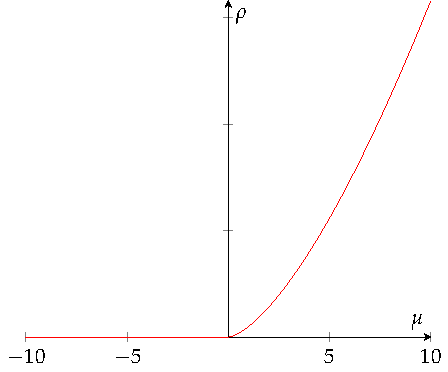
\includegraphics[]{Images/fig-rhomu.pdf}
    
    \caption{Plot of $\rho$ vs. $\mu$ (arbitrary units). $\rho$ is zero for $\mu \leq 0$ and $\rho \propto \mu^{3/2}$ for $\mu > 0$, signalling a phase transition in the system.}
    \label{fig-rhomu}
\end{figure}

The fact that $\rho \propto \mu^{3/2}$ is obtainable by realizing that $k_F \propto \rho^{1/3}$ (Eq. \eqref{eq-kF}) and $\mu = \e_F \propto k_F^2$ (Eqs. \eqref{eq-muef} and the definition of Fermi energy). Since $\phi \propto P \propto u$ (Eqs. \eqref{eq-phi} and \eqref{eq-P}), and $u \propto \rho^{5/3}$ (Eq. \eqref{eq-rho}), we find that the free energy $\phi$ is related to the chemical potential by $\phi \propto \mu^{5/2}$.

Since we have to take three derivatives of $\phi$ w.r.t. $\mu$ before we get a discontinuity (at $\mu = 0$), by the Ehrenfest classification of phase transitions, this is a third order phase transition. This discussion can also be taken as something that highlights the difference between Fermi gas and Fermi liquid behaviour; interactions change the properties of the system significantly.

\end{document}